\scanpage{142}
% archive foliation: 141
$f:X\longrightarrow S$ projectif et lisse, fibres géom connexes de dim 1.

$U=X-Y$, \inserted{p. ex. $Y=$} $[\coprod_{i\in I}g_i(S)$, les $g_i$ des sections telles que les $g_i(S)$ deux à deux disjoints$]$
\margin{$Y$ sous-schéma fermé de $X$ \uline{étale} sur $S$}
\[
f_U:U\mathbin{\text{---}}S
\]
$n$ premier aux car. résiduelles\inserted{ de $S$}. On trouve
\[
E_2^{pq}=H^p(S,\underbrace{R^q_!f_U(\mu_n)}_{\substack{0\text{ sauf si}\\q=1,2}})\Longrightarrow H^*_{\mathrm{prop}}(\unsure{U},\mu_n)
\]
\[
R^q_!f_U(\mu_n)=\begin{cases}
0&\text{si }q\unsure{\notin|\ne}\{1,2\\
{}_n\mathbf E&\text{si }q=1\\
(\mathbf Z/n\mathbf Z)_S&\text{si }q=2
\end{cases}
\]
\margin{(def. de $E$ cf plus bas)}
\figure{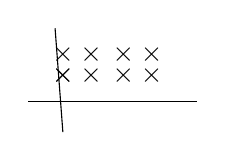
\begin{tikzpicture}[scale=.55]
\draw (-.8,0)--(3.1,0);\draw (0,-.7)--(-.18,1.7);
\foreach \x in {0,.65,1.4,2.05}{\node at (\x,.6) {$\times$};\node at (\x,1.1) {$\times$};}
\node[font=\bfseries] at (0,.6) {$\times$};
\end{tikzpicture}}
\diagram{\begin{tikzcd}
E_2^{02}\arrow[r]\arrow[d,equal]&E_2^{2,1}\arrow[d,equal]\\
H^0(S,\mathbf Z/n\mathbf Z)&H^2(S,{}_n E)
\end{tikzcd}}

On trouve un élément canonique
\[
\xi_n\in H^2(S,{}_n E)
\]
Si $n=\ell^\nu$ ($\nu$ variable), $\ell$ premier distinct des car. rés. sur $S$, on trouve
\[
\boxed{\xi(\ell)\in H^2(S,\mathbf T_\ell(E))}
\]
Cet \uline{élément est nul si} $U$ \uline{a une section sur} $S$.

$\mathbf E$ est un schéma en groupes lisse sur $S$, \deleted{\unsure{et}}\inserted{à fibres connexes}, (extension de $J=\uline{\mathrm{Pic}}^0_{X/S}$ par $T=G_m^I/G_m$\inserted{ $\longrightarrow$ diagonale})
\diagram{\begin{tikzcd}
0\arrow[r]&T\arrow[r]\arrow[d,equal]&\mathbf E\arrow[r]&J\arrow[r]&0\\
&G_{mS}^I/G_{mS}&&&
\end{tikzcd}}

